\documentclass{article}

\usepackage[utf8]{inputenc}
\usepackage[english]{babel}
\usepackage{graphicx}

 
\usepackage[backend=biber]{biblatex}
\addbibresource{sources.bib}

\title{ET4394 Wireless Networking - Analyzing CRC faults}
\date{}
\author{
Bernard Bekker - xxxxxx \\
Bart Rijnders - 4103505
}

\begin{document}

\maketitle

\section{Abstract}

In this report the effect of signal strength, frequency and data rate on the amount of CRC failures in WiFi networks is analyzed. Several hours of data was collected using a laptop with it's WiFi adapter and a python library pyshark. This library is a python wrapper for tshark and allows packet parsing using wireshark dissectors. (insert resultaten)


\section{Hypotheses}

Packet loss can occur when the signal is insufficiently strong

\subsection{SNR vs CRC}

We expect to see a quick dropoff when the signal-to-noise ratio drops below the required SNR value.

\subsection{packet length}
We expect to see a linear amount of errors compared to packet length

\subsection{errors by channel}
We expect to see a difference in errors on different channels, depending on how busy they are.

\subsection{datarates}
We expect to see a higher amount of errors when seeing a low signal combined with a high datarate

\section{Methodology}

We capture packets using an intel wireless dualband-AC 8265. Alternatively, we attempted to capture packets on an ALPHA xxxx external wifi adapter, and a C.H.I.P. ARM devboard with buid in wifi.
TShark was used to capture the packets. A python script was written for channelhopping.


\section{results}

\subsection{signal strength versus crc errors}

\begin{figure}
		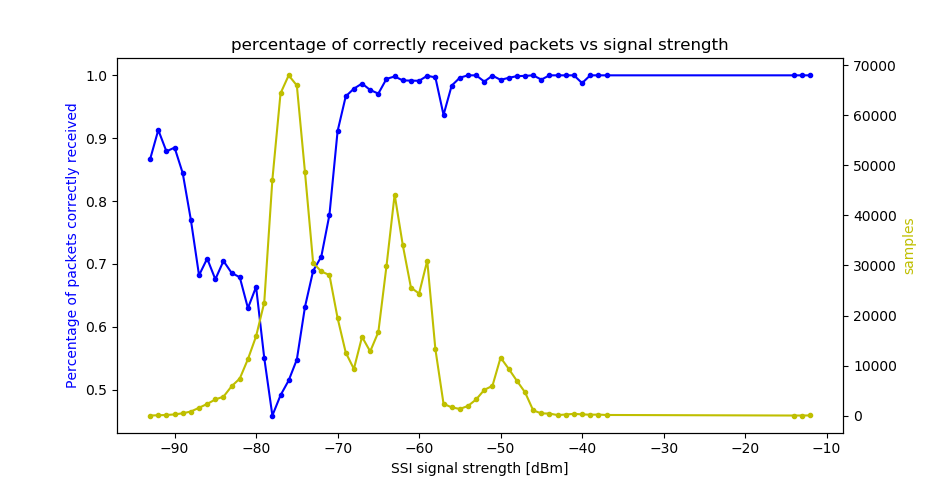
\includegraphics[width=\textwidth]{figures/packets_total.png}
		\caption{}
		\label{fig:totalpackets}
\end{figure}

Some interesting aspects can be seen in figure \ref{fig:totalpackets}. The good reception at high signal strengths, a strong dropoff after a certain point, and two main dips in the reception of correct packets. The most starteling aspect is the rise in correctly received packets at even lower signal strength. We can see more patterns if we split the results into 2.4Ghz channels, and 5.8 Ghz channels (fig \ref{fig:24packets} and fig \ref{fig:58packets}). The two dips are explained by the different dropoff points for 2.4 Ghz and 5.8Ghz. Because 5.8Ghz has less noise, the packets can be correctly demodulated at a lower signal strength.

\begin{figure}
		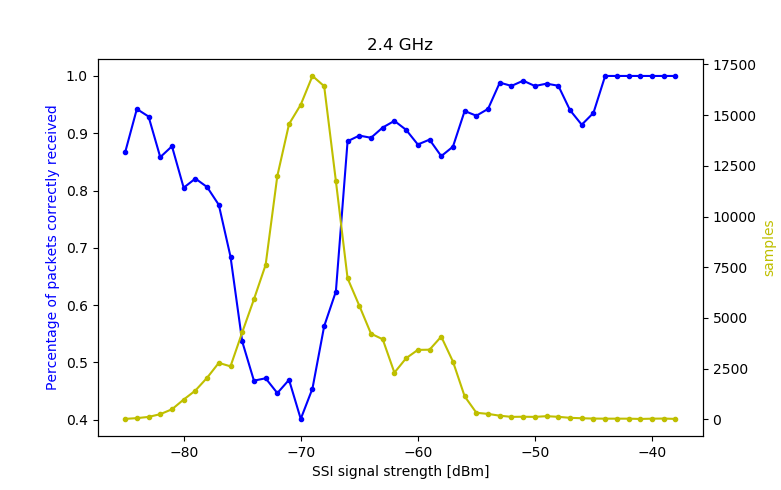
\includegraphics[width=\textwidth]{figures/24ghz.png}
		\caption{}
		\label{fig:24packets}
\end{figure}

\begin{figure}
		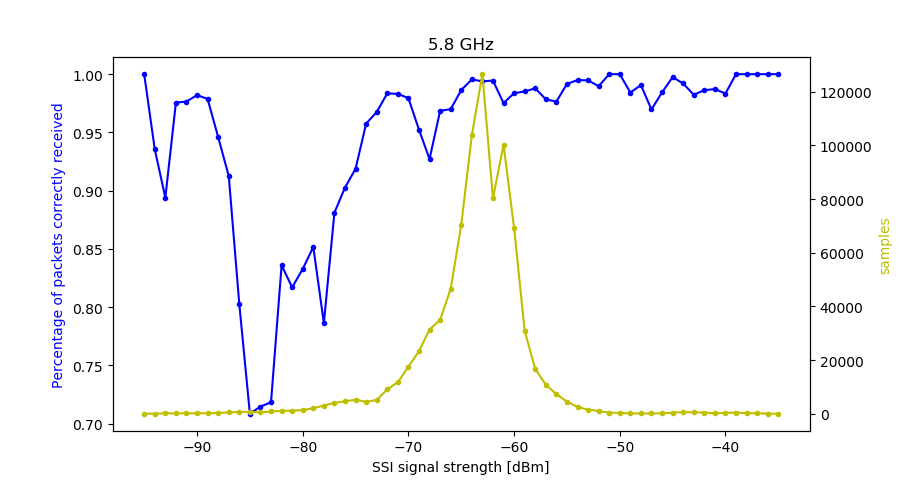
\includegraphics[width=\textwidth]{figures/58ghz.png}
		\caption{}
		\label{fig:58packets}
\end{figure}

This leaves to explain why the graph turns up again at very low signal strenghts. We expect this to be a result of this experiment not being a controlled experiment. Since we do not have a control of what packets are being send, the results only show the packets that are received by the network adapter. When the signal deteriorates too far, it is no longer forwared to the driver and OS. We can see this clearly in fig \ref{fig:datasignal}. At low signal rates, only the packets with a low datarate are returned. (As expected due to Shannon's law)

\begin{figure}
		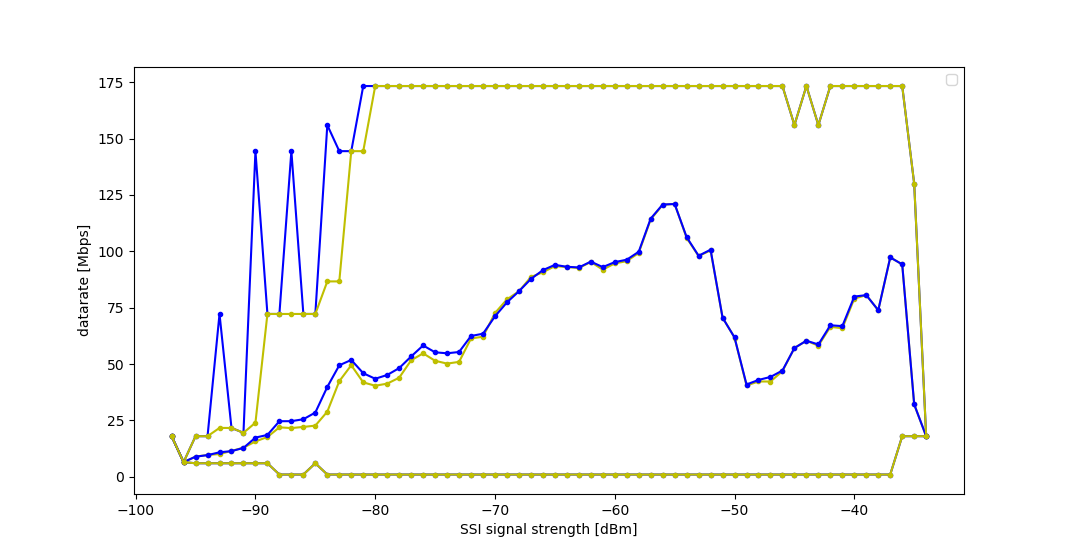
\includegraphics[width=\textwidth]{figures/datarate_signal.png}
		\caption{maximum, mean and minimal reported datarates of received packets vs. signal strength. The blue line is the datarate of all received packets, the green line the datarate of packets without CRC errors. At low signal strenghts, all lines converge as the network adapter drops all undecipherable packets and only shows packets that are succesfully received due to their low datarate.}
		\label{fig:datasignal}
\end{figure}

\subsection{Packet length}
\begin{figure}
		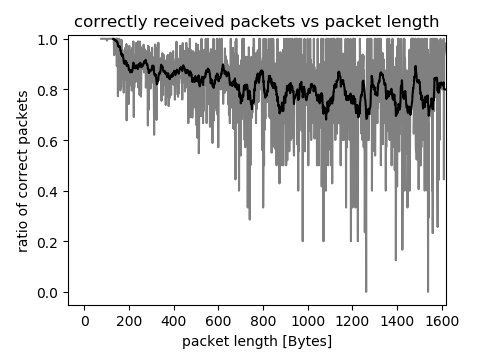
\includegraphics[width=\textwidth]{figures/length.png}
		\caption{Percentage of packets without error versus packet length.}
		\label{fig:datasignal}
\end{figure}


\printbibliography

\end{document}